\documentclass[a4paper,10pt,captions=tableheading,DIV=14]{scrartcl}
\pdfoutput=1

% ----------------------------------------------------------- Packages
\usepackage{amsmath,amssymb,url,cite,slashed,cancel,booktabs,hyperref,graphicx,xspace,subcaption}
\usepackage{braket}
\usepackage[capitalize]{cleveref}
%%%UNUSED%%% \usepackage{feynmp,enumerate,multirow,wrapfig}
\renewcommand\citepunct{,\penalty1000\hskip.13emplus.1emminus.1em\relax} % no line-break in \cite
\renewcommand\thefootnote{*\arabic{footnote}}
\numberwithin{equation}{section}
% COMMENTS
\newcommand{\comment}[1]{{\textbf{\small \color{red} [#1]}}}
\newcommand{\cmark}{\ding{51}} % check mark
\newcommand{\xmark}{\ding{55}} % X mark

% MATH NOTATION
\newcommand\w[1]{_{\mathrm{#1}}}
\newcommand\vc[1]{{\boldsymbol{#1}}}
\newcommand\dd{\mathop{}\!\mathrm{d}}
\newcommand\DD{\mathop{}\!\mathrm{D}}
\newcommand\ee{\mathop{}\!\mathrm{e}}
\newcommand\abs[1]{\lvert#1\rvert}
\newcommand\norm[1]{\lVert#1\rVert}
\newcommand\Abs[1]{\left\lvert#1\right\rvert}
\newcommand\Norm[1]{\left\lVert#1\right\rVert}
\newcommand\ii{\mathrm{i}}
\newcommand\co[1]{\mathrm{c}_{#1}}
\newcommand\si[1]{\mathrm{s}_{#1}}
\newcommand\coco[1]{\mathrm{c}^2_{#1}}
\newcommand\sisi[1]{\mathrm{s}^2_{#1}}
\newcommand\pmat[1]{\begin{pmatrix}#1\end{pmatrix}}
\DeclareMathOperator{\Order}{\mathcal{O}}
\DeclareMathOperator{\sign}{\mathrm{sign}}
\DeclareMathOperator{\ddelta}{\delta}
\DeclareMathOperator{\Tr}{\mathrm{Tr}}
\DeclareMathOperator{\Br}{\mathrm{Br}}
\DeclareMathOperator{\diag}{\mathrm{diag}}
\renewcommand{\Re}{\mathop{\mathrm{Re}}}
\renewcommand{\Im}{\mathop{\mathrm{Im}}}

\newcommand\oneone{1}
\newcommand{\dn}[3]{\frac{\dd^#1 #2}{\dd #3^#1}}    % derivatives
\newcommand{\pdn}[3]{\frac{\partial^#1 #2}{\partial #3^#1}}
\newcommand{\pd}[2]{\frac{\partial #1}{\partial #2}}
\newcommand\parenfrac[3]{\def\temp{#3}\Bigl(\frac{#1}{#2}\Bigr)\ifx\oneone\temp\relax\relax\else^{#3}\fi}
\newcommand\vev[1]{\langle#1\rangle}
\newcommand{\mean}[1]{\left\langle #1 \right\rangle}

\newcommand\hc{\text{h.c.}}

% units
\newcommand\unit[1]{\,\mathrm{#1}\xspace}
\newcommand\eV{\unit{eV}}
\newcommand\keV{\unit{keV}}
\newcommand\MeV{\unit{MeV}}
\newcommand\GeV{\unit{GeV}}
\newcommand\TeV{\unit{TeV}}
\newcommand\PeV{\unit{PeV}}
\newcommand\fb{\unit{fb}}
\newcommand\pb{\unit{pb}}
\newcommand\iab{\unit{ab^{-1}}}
\newcommand\ifb{\unit{fb^{-1}}}
\newcommand\ipb{\unit{pb^{-1}}}
\newcommand\fm{\unit{fm}}


% scientific form of numbers
\makeatletter
\def\EE{\@ifnextchar-{\@@EE}{\@EE}}
\def\@EE#1{\ifnum#1=1 \times\!10 \else \times\!10^{#1}\fi}
\def\@@EE#1#2{\times\!10^{-#2}}
\makeatother

% ---------------------------------------------------- For Sho's Notes
\usepackage{scrlayer-scrpage,color,soul}
\usepackage[hhmmss]{datetime}
\newdateformat{mydate}{\THEDAY\;\shortmonthname.\;\THEYEAR}
\addtokomafont{pagehead}{\small\normalfont}
\ohead{\texttt{[\jobname~@~\mydate\today~\currenttime]}}
\bibliographystyle{utphys27mod}

% --- minted experimental
\usepackage{ifplatform,listings}
\lstset{columns=[l]fullflexible,basicstyle=\small\ttfamily,xleftmargin=2em,frame=L,keepspaces=true}
\ifshellescape
\usepackage{minted}
\setminted{linenos,xleftmargin=7\fboxsep,breaklines,fontsize=\small,frame=leftline,stepnumber=5,framesep=2\fboxsep,escapeinside=||,mathescape=true}
\setminted[console]{xleftmargin=6\fboxsep,frame=none}
\else
\makeatletter
\lstnewenvironment{minted}[1]
  {\csname\@lst @SetFirstNumber\endcsname}
  {\csname\@lst @SaveFirstNumber\endcsname}
\makeatother
\fi
% ---

\newcommand{\mathfunc}[2]{\mathcmd{#1}\texttt{[}\matharg{#2}\texttt{]}}
\newcommand{\mathcmd}[1]{\textup{\texttt{#1}}}
\newcommand{\mathtext}[1]{\textup{\texttt{"#1"}}}
\newcommand{\matharg}[1]{\textsl{#1}}

\newcommand{\TODO}[1]{{\textbf{\lstset{}\color{red}$\clubsuit$#1}}}

% commands for this document
\newcommand\doi[1]{{\footnotesize \texttt{\href{https://doi.org/#1}{[#1]}}}}
\definecolor{navy}{rgb}{0,0,0.5}
\newcommand\Damu{\Delta a_\mu}
\newcommand\amu[1][\relax]{\ifx#1\relax{a_\mu}\else{a_\mu^{\mathrm{#1}}}\fi}
\newcommand\smu{\tilde\mu}
\newcommand\smuL{\tilde\mu\w L}
\newcommand\smuR{\tilde\mu\w R}
\newcommand\lL{\tilde l\w L}
\newcommand\lR{\tilde l\w R}
\newcommand\neut  [1][\relax]{{\tilde\chi^0_{#1}}}
\newcommand\charP [1][\relax]{{\tilde\chi^+_{#1}}}
\newcommand\charM [1][\relax]{{\tilde\chi^-_{#1}}}
\newcommand\charPM[1][\relax]{{\tilde\chi^\pm_{#1}}}
\newcommand\file[1]{\lstinline[basicstyle=\ttfamily\color{navy}]{#1}}
\newcommand\package[2][\relax]{\texttt{#2}\ifx#1\relax\relax\else~\texttt{#1}\fi}
\newcommand\mET{\cancel{E}\w T}

\newcommand{\gL}{g\w L}
\newcommand{\gR}{g\w R}
\newcommand{\PL}{P\w L}
\newcommand{\PR}{P\w R}

\newcommand{\thuz}{\tilde h\w u^0}
\newcommand{\thdz}{\tilde h\w d^0}
\newcommand{\thup}{\tilde h\w u^+}
\newcommand{\thdm}{\tilde h\w d^-}

\author{Sho Iwamoto}
\title{Details of each benchmark line}
\begin{document}
%\maketitle
\begin{center}{\makeatletter
{\huge\usekomafont{title}\@title}\par\vspace{2em}
{\Large \@author}\par\vspace{2em}
}
\begin{abstract}\noindent
Details (fail safe note) for each of my analyses.
\end{abstract}
\end{center}

%---------------------------------------------------------------------

\section{Prerequisites}
\subsection{Decay chain and accepted signal categorization}
We use the following notation for (s)leptons to avoid confusion in this note (but possibly be avoided in the paper).
\begin{align*}
\lL &= (\tilde e\w L, \tilde \mu\w L, \tilde\tau\w L),
&
\tilde\nu &= (\tilde \nu_e, \tilde\nu_\mu, \tilde\nu_\tau),
&
\text{slepton}=(\lL,\tilde\nu, (\lR)),
\\
l&=(e,\mu,\tau),
&
\ell&=(e,\mu),\dots
\end{align*}
In addition, to reinterpret LHC analyses, we use the following labels for simplified models (``chain''s):
\begin{align}
 \text{NC/3L}&: \neut\charPM\to
\left[
\Bigl(\lL^{(*)}l^{(*)},\tilde\nu^{(*)}\tilde\nu^{(*)};\text{1/12 each}\Bigr)
\Bigl(\tilde\nu l,\lL\nu;\text{1/6 each}\Bigr)
\right]
 \otimes(\text{slep}\to \text{lep}\neut[\text{LSP}]; \text{100\%})\\
 \text{NC/LLT}&: \neut\charPM\to
\left[
\Bigl(\lR^{(*)}l^{(*)};\text{1/6 each}\Bigr)
\Bigl(\tilde \tau\w R\nu;\text{100\%}\Bigr)
\right]
 \otimes(\text{slep}\to \text{lep}\neut[\text{LSP}]; \text{100\%})\\
\text{NC/3T}&: \neut\charPM\to
\left[
\Bigl(\tilde\tau\w R^{(*)}\tau^{(*)};\text{1/2 each}\Bigr)
\Bigl(\tilde \tau\w R\nu;\text{100\%}\Bigr)
\right]
 \otimes(\text{slep}\to \text{lep}\neut[\text{LSP}]; \text{100\%}),\\
 \text{NC/WZ}&: \neut\charPM\to(Z\neut[\text{LSP}])(W^\pm\neut[\text{LSP}])~~\text{(possibly virtual)},\\
 \text{NC/WH}&: \neut\charPM\to(H\neut[\text{LSP}])(W^\pm\neut[\text{LSP}])~~\text{(possibly virtual)},\\
 \text{CC/2L}&: \charP\charM\to
\left[
\Bigl(\tilde\nu l^*,\lL^*\nu;\text{1/6 each}\Bigr)
\Bigl(\tilde\nu^* l,\lL\nu^*;\text{1/6 each}\Bigr)
\right]
 \otimes(\text{slep}\to \text{lep}\neut[\text{LSP}]; \text{100\%}),\\
 \text{SLSL}&: (\lL\lL^*\text{ or }\lR\lR^*;\text{6 particles degen.})
 \otimes(\text{slep}\to \text{lep}\neut[\text{LSP}]; \text{100\%}),
% \text{CC/WW}&: \charP\charPM\to(W^+\neut[\text{LSP}])(W^-\neut[\text{LSP}])~~\text{(possibly virtual)},
\end{align}
where the virtual $Z$, $W^\pm$, and $H$ are assumed to decay according to the SM theoretical branching ratio.

\subsection{Our approximation}

In SUSY searches by the ATLAS and CMS collaborations, they represent the results in several ways.
The 95\% confidence upper limit on production cross section, $\sigma\w{UL}$, is one of such forms, where a simplified SUSY scenario and particular production processes are considered and consistency with the Standard Model is given by the upper limit on the production cross section of the particular processes.
A model is excluded with 95\% confidence level if $\sigma\w{UL}$ is smaller than the theoretical cross section $\sigma\w{theory}$.

If $\sigma\w{UL}$ is calculated from one signal region (SR), it is related to the upper limit on the number of events in the SR, $N\w{UL}$, by
\begin{equation}
 \frac{N\w{UL}}{\mathcal L} = (\mathcal A\cdot \mathcal E)\cdot\sigma\w{UL;original}.
\label{eq:NUL}
\end{equation}
Here, we introduce a label ``original'' to clarify that the limit is for their original simplified scenario.
The left-hand side is independent of the processes or models, where $\mathcal L$ is the integrated luminosity, while the process dependence is contained in the acceptance $\mathcal A$ and efficiency $\mathcal E$.
Therefore, their result can be applied to any models $X$ if we calculate the acceptance and efficiency for the model $X$; specifically, we should compare $\sigma_{X;\text{theory}}$ with
\begin{equation}
 \sigma_{\text{UL};X} :=
 \frac{(\mathcal A\cdot \mathcal E)\w{original}}{(\mathcal A\cdot\mathcal E)_X}\cdot\sigma\w{UL;original}.
\label{eq:ULtranslation}
\end{equation}
$(\mathcal A\cdot\mathcal E)_{X}$ however requires Monte Carlo simulation with full detector simulation.
To avoid such complexity, we approximate the ratio by, assuming that $X$ is similar to the original process,
\begin{equation}
 \frac{(\mathcal A\cdot \mathcal E)\w{original}}{(\mathcal A\cdot\mathcal E)_X}
\approx
 \frac{A\w{original}}{A_X}=:\frac{1}{K_\Gamma},
\label{eq:ULapprox}
\end{equation}
where $A$, simplified acceptance, is calculated just from the decay ratios of the relevant particles.

The above procedure is less justifiable if $\sigma\w{UL;original}$ is given by statistical combination of multiple SRs\footnote{Mainly because of the approximation $\mathcal E\w{original}/\mathcal E_X\approx 1$.},
but we will apply it as far as the expression of $A$ is common for, or at worst, the values of $K_\Gamma$ are similar for, the SRs combined.

Then, this upper limit is compared with the theoretical production cross section $\sigma_X$:
\begin{equation}
 \sigma_X \text{~~v.s.~~} \sigma_{\mathrm{UL};X}=\frac{A\w{original}}{A_X}\sigma\w{UL;original}.
\end{equation}
Note that these variables have physical sense.
There is an equivalent comparison,
\begin{equation}
 A_X \sigma_X \text{~~v.s.~~} A\w{original}\sigma\w{UL;original},
\end{equation}
which may be useful in some cases because the model dependence is contained in one side.




\section{LHC Analyses}
\subsection{ATLAS 1803 (36/fb)}
ATLAS 1803\cite{1803.02762} has the following analyses\footnote{``SF'', ``OS'', ``SS'' are respectively for same flavor, opposite sign, and same sign. $(3\ell)\w{SFOS}$ means that two of them form a SFOS pair and the other is arbitrary. Particles are ``hard'' (not soft) unless noted as such. Events with extra leptons are vetoed in some analyses, but I do not care those vetoes as we are anyway not interested in events to be vetoed.}:
\begin{itemize}
 \item[(a)] CC/2L(0.5) --- $(2\ell)\w{OS}0j$ --- Fig. 8(a) \doi{10.17182/hepdata.81996.v1/t78}
 \item[(b)] SLSL       --- $(2\ell)\w{OS}0j$ --- Fig. 8(b) \doi{10.17182/hepdata.81996.v1/t79}
 \item[(c)] NC/3L(0.5) --- $(3\ell)\w{SFOS}$  --- Fig. 8(c) \doi{10.17182/hepdata.81996.v1/t80}
 \item[(d)] NC/WZ      --- $(3\ell)\w{SFOS}\oplus(2\ell)\w{SFOS}2j$  --- Fig. 8(c) \doi{10.17182/hepdata.81996.v1/t81},
\end{itemize}
where the first (second) column shows the considered chains (signal regions for the analysis), the third column gives the references to the exclusion plot on the paper, and the last column shows the DOIs to the data resources of $\sigma\w{UL}$.

Since our scenarios with $x=0.50$ is similar to the model NC/3L(0.5), reinterpretation of their analysis (c) will give an estimation of LHC bounds to them.
Noting the requirement of SFOS pair, the probability that chain-NC/3L with $x=0.5$ produces signatures falling in the category is estimated by
\begin{equation}
\label{eq:tau-3L-3L0.5}
 p\Bigl((3\ell)\w{SFOS}\Big|\text{NC/3L}(0.5)\Bigr)\approx
\left[
 p(\tilde\ell,\tilde\nu_\ell|\charPM[1])
+ p_\ell \cdot p(\tilde\tau,\tilde\nu_\tau|\charPM[1])
\right]
\left[
 p(\tilde\ell^{(*)}|\neut[2])
+ \frac{3p_\ell^2}{4} \cdot p(\tilde\tau^{(*)}|\neut[2])
\right],
\end{equation}
which we will use the simplified acceptance $A(\text{ATLAS1803c})$.
Here, $p_\ell\simeq0.352$ is the leptonic decay rate of $\tau$.
Also note that, here and hereafter, $\Br(\text{slep}\to\text{lep}+\neut[1])=1$ (as well as flavor conservation) is assumed.

We similarly obtain the expressions of $A$ for the other analyses. The result is summarized as
\begin{align}
 A(\text{ATLAS1803b}) &= 1,
\\
 A(\text{ATLAS1803c}) &=  \left[
 p(\tilde\ell,\tilde\nu_\ell|\charPM[1])
+ p_\ell \cdot p(\tilde\tau,\tilde\nu_\tau|\charPM[1])
\right]
\left[
 p(\tilde\ell^{(*)}|\neut[2])
+ \frac{3p_\ell^2}{4}\cdot p(\tilde\tau^{(*)}|\neut[2])
\right],
\\
 A(\text{ATLAS1803d}) &=
 \Br(\charPM[1]\to W^\pm\neut[1])
 \Br(\neut[2]\to Z\neut[1]).
\end{align}
Here one should note that, though $\sigma\w{UL}$ for (d) is calculated by statistical combination of two very different signal categories, the expression of $A$ is common for those two categories and hence we will use it.
Also,
\begin{align}
 A(\text{ATLAS1803b})\w{original} &= 1,\\
 A(\text{ATLAS1803c})\w{original} &=
\left(\frac46 + \frac26p_\ell\right)\left(\frac{4}{12}+\frac{3p_\ell^2}{4}\frac{2}{12}\right)=0.273,\\
 A(\text{ATLAS1803d})\w{original} &= 1.
\end{align}

\clearpage

\subsection{CMS 1709 (36/fb)}
We use the following analyses in CMS1709\cite{1709.05406}:
\begin{itemize}
 \item[(a)]  NC/3L(0.5)            --- $(3\ell)\w{SFOS}$                           --- Fig.~14
 \item[(b)]  NC/3L(0.05, 0.95)     --- $(3\ell)\w{SFOS}\oplus(2^=\ell)\w{SS}$      --- Fig.~15a, 15b
 \item[(b1)] NC/3L(0.05, 0.95)     --- $(2^=\ell)\w{SS}$      --- Aux.~Fig.~1, 3
 \item[(b2)] NC/3L(0.05, 0.95)     --- $(3\ell)\w{SFOS}$      --- Aux.~Fig.~2, 4
 \item[(c)]  NC/LLT(0.05,0.5,0.95) --- $(3\ell)\w{SFOS}\oplus(2\ell)\w{SFOS}1\tau$ --- Fig.~16a, 16c, 16b
 \item[(c1)] NC/LLT(0.05,0.5,0.95) --- $(3\ell)\w{SFOS}$      --- Aux.~Fig.~7, 5, 9
 \item[(c2)] NC/LLT(0.05,0.5,0.95) --- $(2\ell)\w{SFOS}1\tau$ --- Aux.~Fig.~8, 6, 10
 \item[(d)]  NC/WZ                 --- $(3\ell)\w{SFOS}$  --- Fig.~18a
 \item[(e)]  NC/WH                 --- various signatures --- Fig.~18b
\end{itemize}
The data are provided in \texttt{.root} format at \url{http://cms-results.web.cern.ch/cms-results/public-results/publications/SUS-16-039/}.
Note that we use (b1), (b2), etc., whose data are provided in auxiliary plots, instead of (b) etc.\ because of the lack of reasonable $A$.
We use, as the simplified acceptances,
\begin{align}
 A(\text{CMS1709a}) &=  A(\text{ATLAS1803c}), \quad\vev{0.273}\\
 A(\text{CMS1709b2}) &=  A(\text{ATLAS1803c}), \quad\vev{0.273}\\
 A(\text{CMS1709c1}) &= A(\text{ATLAS1803c}), \quad\vev{0.246}\\
\begin{split}
  A(\text{CMS1709c2}) &=
  \frac{p\w hp_\ell^2}{2} p(\tilde\tau^{(*)},\tilde\nu_\tau^{(*)}|\charPM[1])p(\tilde\tau^{(*)}|\neut[2])
 + {p\w h} p(\tilde\tau^{(*)},\tilde\nu_\tau^{(*)}|\charPM[1])p(\tilde\ell^{(*)}|\neut[2])
 \\&\qquad
 + \frac{p\w hp_\ell}{2} p(\tilde\ell^{(*)},\tilde\nu_\ell^{(*)}|\charPM[1])p(\tilde\tau^{(*)}|\neut[2]),
 \quad\vev{0.445}
\end{split}\\
A(\text{CMS1709d}) &= A(\text{ATLAS1803d}),\quad\vev{1}\\
 A(\text{CMS1709e}) &= \Br(\charPM[1]\to W^\pm\neut[1]) \Br(\neut[2]\to H\neut[1]),\quad\vev{1}
\end{align}
where the values in $\vev{\cdot}$ is the original values.

\subsection{CMS1807 (36/fb) also SUS-17-002-PAS}
CMS 1807.02048\cite{1807.02048} targets $2\tau+\mET$ signatures.
\begin{itemize}
 \item[(-)] $pp\to\tilde\tau\tilde\tau$ --- no constraints are obtained.
 \item[(a)] NC/3T(0.5) --- $e\tau_h, \mu\tau_h, e\mu, \tau_h\tau_h$ --- Fig.~14
 \item[(b)] CC/2T(0.5) --- $e\tau_h, \mu\tau_h, e\mu, \tau_h\tau_h$ --- Fig.~15
\end{itemize}
We use, as the simplified acceptance,
\begin{align}
 A(\text{CMS1807a}) &=
 p(\tilde\tau^{(*)},\tilde\nu_\tau^{(*)}|\charPM[1])
 p(\tilde\tau^{(*)}|\neut[2]),\quad\vev{1}\\
 A(\text{CMS1807b}) &=
 p(\tilde\tau^{(*)},\tilde\nu_\tau^{(*)}|\charPM[1])^2.\quad\vev{1}
\end{align}
We simply neglect contributions from decays such as $\neut[2]\to\ell\tilde\ell$ for simplicity and conservativeness.

This paper is a combination of CMS-PAS-SUS-17-002 and 003. CMS-PAS-SUS-17-002 also analyzes different $x$, but necessary data are not provided and we do not use it:\footnote{The CMS collaboration wrote ``equal branching fractions assumed for each of the two possible $\charPM[1]$ decay chains'' in the paper version, while such comments are not found in the PAS version. Thus SI thinks that the PAS analysis (c) is done with assuming $\Br(\charM[1]\to\tilde\tau\bar\nu)=1$; the very different shapes of Fig.~10(a,c) supports this consideration.
The published analysis (a) may possibly be done with $\Br(\charM[1]\to\tilde\tau\bar\nu)=1$ (while we assume they did with 0.5) but this difference does not affect as far as $m_{\tilde\tau_1}\simeq m_{\tilde\nu_\tau}$.}
\begin{itemize}
 \item[(-)] NC/3T(0.05,0.95) --- $e\tau_h,\mu\tau_h,e\mu$ -- Fig.~10(a,c).
\end{itemize}

\subsection{ATLAS1806 (36/fb)}
ATLAS 1806.02293\cite{1806.02293} uses the same dataset as ATLAS1803 and focuses on $WZ+\mET$ search with elaborated selections.
Cross section upper limits are available as:
\begin{itemize}
 \item NC/WZ --- $(2^=\ell2j)\oplus(3^=\ell)$ --- Fig.~13c (Aux.~Fig.~18c)
\doi{10.17182/hepdata.83419.v1/t41}
\end{itemize}


\subsection{ATL-CONF-2019-020 (139/fb)}
ATLAS-CONF-2019-020 focuses NC/WZ signature with $M_2-M_1 \gtrsim m_Z$ semi-compressed region.
The exclusion is limited to $m_{\charPM[1]}<350\GeV$ and no limits are given for $m_{\neut[1]}>0.5m_{\charPM[1]}$.
So I estimate that we do not have to consider this analysis.\footnote{I once wrote ``Note that the importance of this search on our models cannot be estimated without HEPData.'', considering that this result may matter, but I do not remember why.}

Anyway, we do not include ATL-CONF-2019-020 in the analysis because HEPData is not given.



\subsection{ATLAS1909 (139/fb; superseding ATLAS1812: 36/fb)}
ATLAS 1812.09432\cite{1812.09432} searches for $Wh+\mET$ signature targetting $Wh\to 0lb\bar b$, $1lb\bar b$, $1l\gamma\gamma$, and $l^\pm l^\pm$, where $0lb\bar b$ gives the stringent limit for $M_2\lesssim500\GeV$ and $1lb\bar b$ does for $M_2\gtrsim500\GeV$.

ATLAS 1909.09226\cite{1909.09226} concentrates on $Wh\to1lb\bar b$ signature and with $139\ifb$ supersedes all the 1812 limit, i.e., it gives better sensitivity than each of the 1812 analyses.
Thus it is sufficient to consider ATLAS1909 here.

\begin{itemize}
 \item NC/Wh --- $(1^=\ell2^=b 1^\le j)$ --- Fig.~6 (Aux.~Fig.~3) \doi{10.17182/hepdata.90607.v1/t17}
\end{itemize}



\subsection{CMS 1801 (36/fb)}
We use the following analyses in CMS 1801.03957\cite{1801.03957}:
\begin{itemize}
 \item[(a)]  NC/WZ                 --- various signatures --- Fig.~8a
 \item[(b)]  NC/WH                 --- various signatures --- Fig.~8b
\end{itemize}
with published root data files on \url{http://cms-results.web.cern.ch/cms-results/public-results/publications/SUS-17-004/}.
These results supersedes CMS1709 (d) and (e).

\subsection{ATLAS 1908 (139/fb)}
We use ATLAS 1908.08215\cite{1908.08215} to constrain the models by $2\ell+\mET$ search. (Thus we do not consider ATLAS1803(a,b), which should be superseded by this search.)

\begin{itemize}
 \item [(-)] CC/2L --- $(2^=\ell1^\le j)$ --- no constraints for $M_1=M_2/2$ \TODO{how about $\mu=0.75M_2$ case?}
 \item [(a)] SLSL --- $(2^=\ell1^\le j)$ --- Fig.~7c (Aux.~Fig.~3c) \doi{10.17182/hepdata.89413.v1/t47}
\end{itemize}


\clearpage

\section{Validation}
As shown in Eq.~\eqref{eq:NUL}, $\mathcal A\mathcal E\sigma\w{UL}$ is unique for each SR and independent of hypothesized models.
If an SR is used in multiple analyses, we can check the validity of our approximation, Eq.~\eqref{eq:ULapprox}, by comparing $A\sigma\w{UL}$ among the analyses.


\begin{figure}[h]
 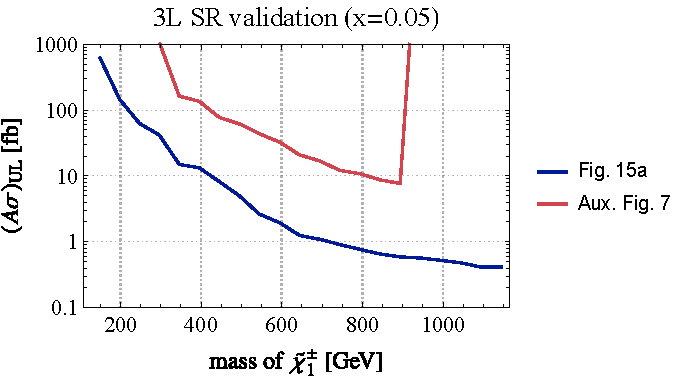
\includegraphics[width=0.33\textwidth]{../plots/validation_cms1709_SRA_tab1_005.pdf}
 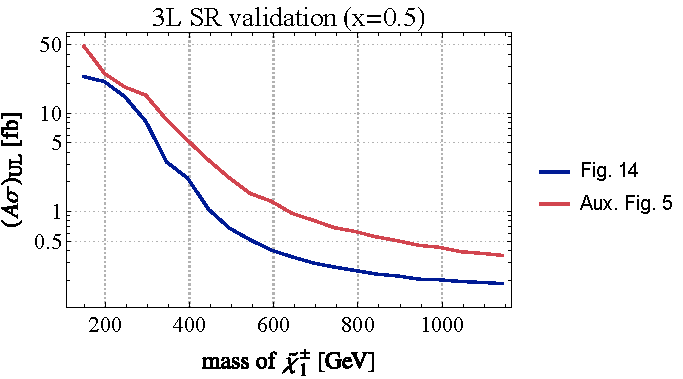
\includegraphics[width=0.33\textwidth]{../plots/validation_cms1709_SRA_tab1_050.pdf}
 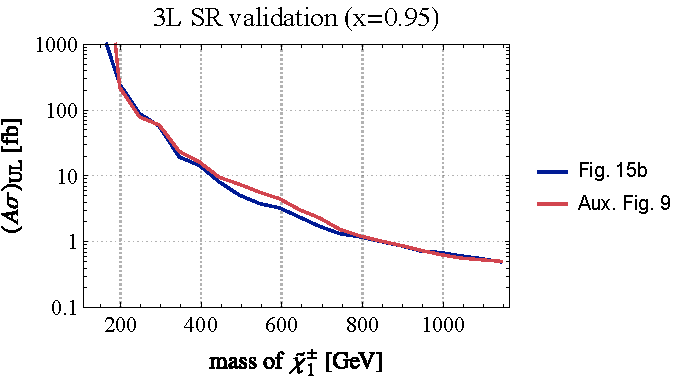
\includegraphics[width=0.33\textwidth]{../plots/validation_cms1709_SRA_tab1_095.pdf}
 \caption{\label{fig:valCMS1709}Comparison of $A\sigma\w{UL}$ for CMS 1709 $(3\ell)\w{SFOS}$ analyses. Dark-blue lines are of (a) and (b2) analyses for NC/3L chain, for which $A=0.273$. Red  ones are of (c1) for NC/LLT chain, for which $A=0.246$.}
\end{figure}


\subsection{CMS1709}
We can perform the validation for $(3\ell)\w{SFOS}$ analysis (the SR``3LA'' in the original paper) by comparing (a) or (b2) with (c1).
The results are shown in \cref{fig:valCMS1709}.
Discrepancies are found in $x=0.05$ and $x=0.5$ cases.

The discrepancy in $x=0.5$ case is probably due to the momentum difference of $\ell$:
\begin{align}
 p\w T(\text{3L}) &\sim 0.5\cdot\Delta m(\charPM[1],\neut[1])\sim 0.25\charPM[1],
&
 p\w T(\text{3L}) &\sim \frac{0.5}{3}\cdot\Delta m(\charPM[1],\neut[1])\sim 0.083\charPM[1].
\end{align}
While the $p\w T$ threshold is 10--25\,GeV, this may give a factor 2--3 difference.

A worse discrepancy is observed in $x=0.05$ case, which is probably caused by the CMS hypothesized model: they assume $\Br(\charPM[1]\to\tilde\tau^\pm\nu^{(*)})=1$ in the LLT case, while in 3L case (as well as our model points) $\Br(\charPM[1]\to\tilde\tau^\pm\nu^{(*)})\sim\Br(\charPM[1]\to\tilde\nu^{(*)}\tau^\pm)$.
The same argument works for $x=0.95$; the resemblance in the plot is just by accident.

\clearpage

\section{Line-by-line analysis}
\subsection{tab1-0.50}

\begin{figure}[h]
  \centering
  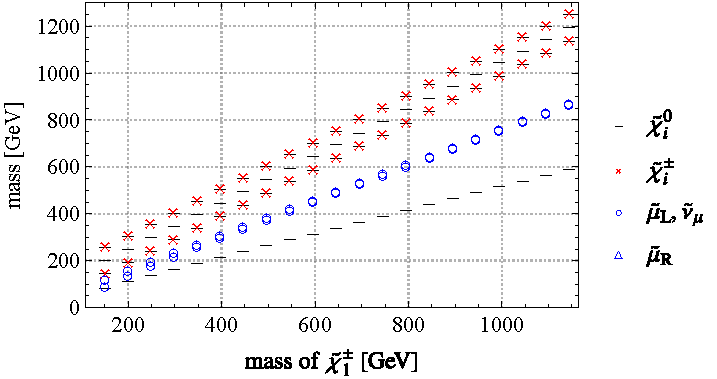
\includegraphics[height=115pt]{../plots/plot_tab1x050_mass.pdf}
  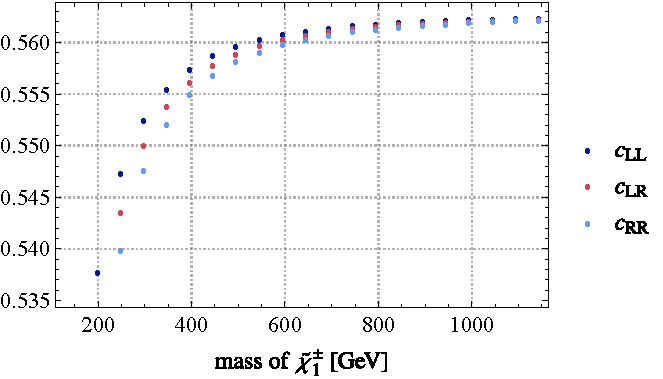
\includegraphics[height=115pt]{../plots/plot_tab1x050_cfactors.pdf}
\par
  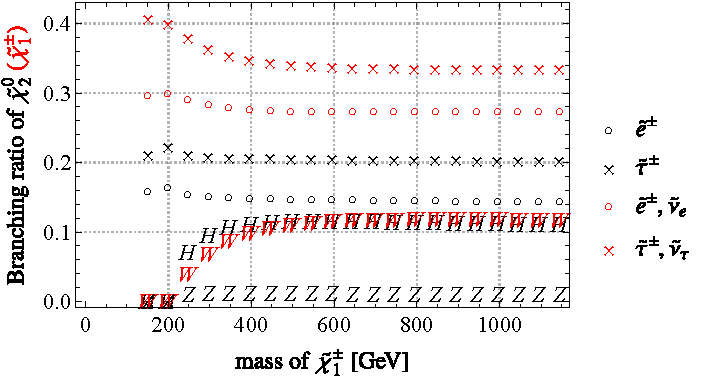
\includegraphics[height=115pt]{../plots/plot_tab1x050_br21.pdf}
  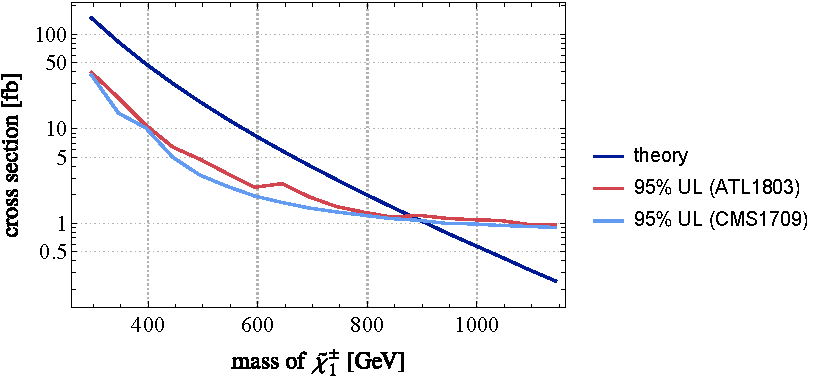
\includegraphics[height=115pt]{../plots/plot_tab1x050_limit.pdf}

  \caption{\label{fig:tab1x050}The property of tab1-0.50 benchmark line. The models are generated with $M_2=200,250,\dots,1200\GeV$, while $m_{\charPM[1]}$ is used as labels.\\
 (A) Masses of relevant SUSY particles. Note that $\tilde\mu\w R$ is decoupled.\\
 (B) The cross-section $c$-factor (see \texttt{analysis.pdf}).\\
 (C) The BRs of $\charPM[1]$ (red) and $\neut[2]$ (black). The bottom black points are ``$H$'' and ''$Z$'' overlapped.\\
 (D) The theoretical cross section and interpreted upper limits on it.
}
\end{figure}

This line is characterized by
\begin{equation}
 M_2=\mu=2M_1,
\quad
 x = \frac{m_{\tilde l\w L}-m_{\neut[1]}}{m_{\neut[2]}-m_{\neut[1]}}=0.5,
\quad
 \tan\beta=40,
\quad
 \tilde l\w R, \tilde q, \text{heavy-Higgs: decoupled}.
\end{equation}

The mass spectrum is shown in \cref{fig:tab1x050}; we use $m_{\charPM[1]}$ to label each model point.
For $m_{\charPM[1]}>300\GeV$, the LSP is $\neut[1]$ and $\neut[2,3,4]\charPM[1,2]$ may give NC/3L-chain.
Meanwhile, we do not consider points with $m_{\charPM[1]}<300\GeV$ as neither by ATLAS.
We safely ignore $\neut[3]$ because of non-degeneracy and smaller production rate, as it has less $\tilde W$-component.
A degenerate pair $\neut[4]\charPM[2]$ may serve as the chain-3L target, but since we have no way to include its contribution, we ignore it, which has a smaller production rate.
Hence, we consider only the NC/3L chain produced by $pp\to\neut[2]\charPM[1]$.

The cross section is, since the $c$-factors are similar for $m_{\charPM[1]}>300\GeV$, given by
\begin{equation}
 \sigma(pp\to\neut[2]\charPM[1])\approx K_{\sigma}\cdot \sigma(pp\to\tilde W^\pm\tilde W^3);
\qquad
 K_\sigma = \mathop{\mathrm{mean}}(c\w{LL},c\w{LR},c\w{RR}),
\end{equation}
where the pure-wino production cross section $\sigma(pp\to\tilde W^\pm\tilde W^3)$ is taken from LHCSUSYXSWG\footnote{\url{https://twiki.cern.ch/twiki/bin/view/LHCPhysics/SUSYCrossSections13TeVn2x1wino}}.

The results against ATLAS1803 is shown in \cref{fig:tab1_x050_atlas1803}, where the black dots correspond to $K_\sigma K_\Gamma \sigma(\text{Wino})$.
It shows that the ATLAS1803 analysis nearly excludes below $\sim860\GeV$.
The wiggles in $\sigma\w{UL}$ is due to interpolation of the $\sigma\w{UL}$-grid ATLAS provides, for which logarithmic interpolation (i.e., linear interpolation on the function $\log\sigma\w{UL}(m_{\charPM[1]},m_{\neut[1]})$) is used.

We may discuss the validity of our approximation consulting \cref{fig:valCMS1709} for $x=0.5$, where our $\sigma\w{UL}$ may be aggressive by factor 2 at worst.
It is however too pessimistic, as the electroweakino decay branch are approximately flavor-democratic. As $\Br(\charPM[1]\to\tilde\tau^\pm) / \Br(\charPM[1]\to\tilde e^\pm) \sim 1.3$, 30\% uncertainty will be enough in this case.

\subsection{tab1-0.05}

\begin{figure}[h]
  \centering
  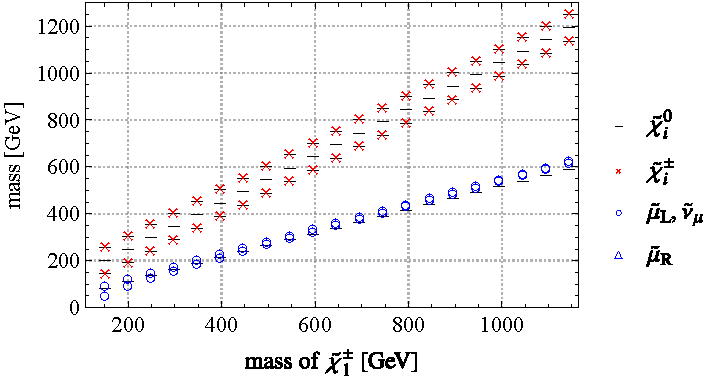
\includegraphics[height=115pt]{../plots/plot_tab1x005_mass.pdf}
  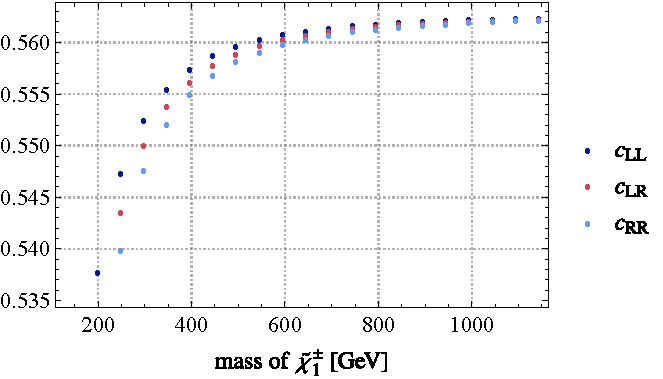
\includegraphics[height=115pt]{../plots/plot_tab1x005_cfactors.pdf}
\par
  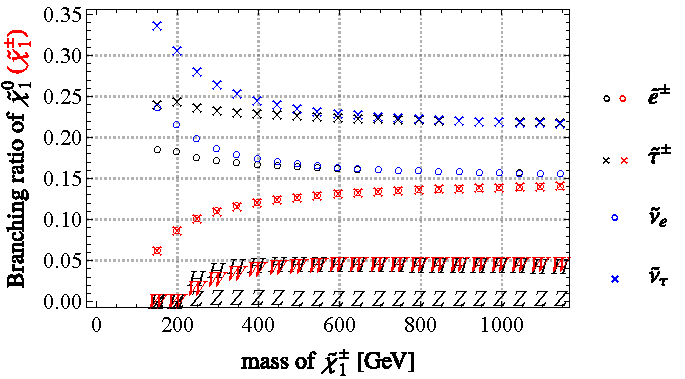
\includegraphics[height=115pt]{../plots/plot_tab1x005_br21.pdf}
  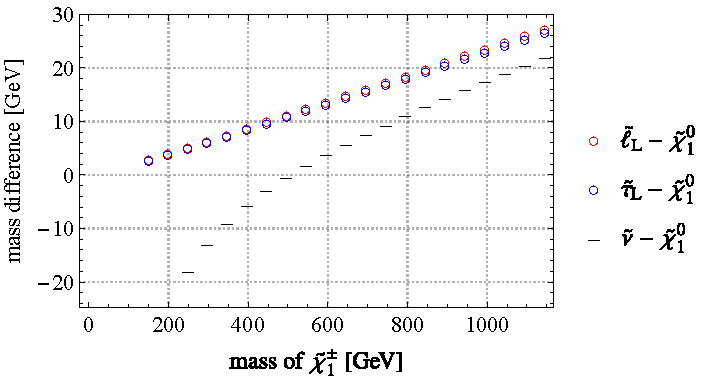
\includegraphics[height=115pt]{../plots/plot_tab1x005_massdiff.pdf}
\par
  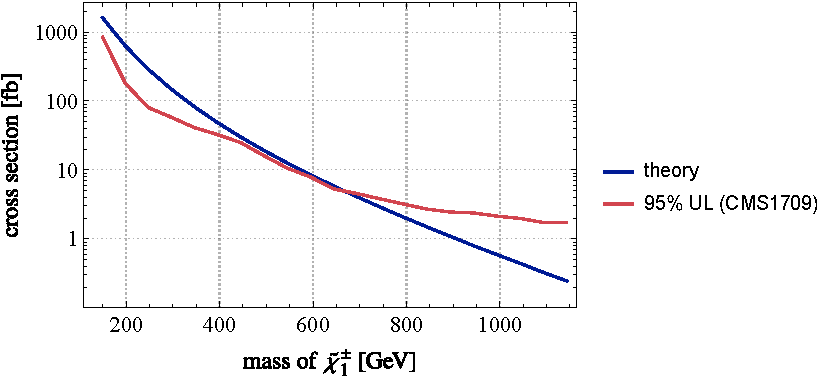
\includegraphics[height=115pt]{../plots/plot_tab1x005_limit.pdf}

  \caption{\label{fig:tab1x005}The property of tab1-0.50 benchmark line. The models are generated with $M_2=200,250,\dots,1200\GeV$, while $m_{\charPM[1]}$ is used as labels.\\
 (A) Masses of relevant SUSY particles. Note that $\tilde\mu\w R$ is decoupled.\\
 (B) The cross-section $c$-factor (see \texttt{analysis.pdf}).\\
 (C) The BRs of $\charPM[1]$ (red/blue) and $\neut[2]$ (black). See text for details since this plot is too complicated.\\
 (D) The mass differences between SUSY particles. The LSP is  $\tilde\nu$ for $m_{\charPM[1]}\lesssim 500\GeV$.\\
 (E) The theoretical cross section and interpreted upper limits on it.
}
\end{figure}


As in the previous case, we focus on $\neut[2]\charPM[1]$ production and calculate the cross section.
The LSP is $\neut[1]$ ($\tilde\nu$) for $m_{\charPM[1]}\gtrsim500\GeV$ ($\lesssim500\GeV$).
At the collider, however, the LSP does not matter much because $\tilde l^\pm$ mainly decays to $\neut[1]$ and it is invisible even if it is not the LSP.
One may claim that the $\tilde\nu$-LSP will, or actually the mass between $\tilde l^\pm$ and $\tilde\nu$, which is not included in the LHC analyses, will, increase $\mathcal A\cdot\mathcal E$ because the resulting $\ell$ will have larger $p\w T$.

\Cref{fig:tab1x005} (C) shows the branching ratios of $\neut[2]$ and $\charPM[1]$.
Focusing on the black points, we see $\neut[2]$ slightly prefer $\tilde\tau\tau$ to $\tilde\ell\ell$.
Meanwhile, $\charPM[1]$ (non-black points) prefers $\tilde\nu_\tau\tau$ to $\tilde\nu_\ell\ell$ but the ratios to charged sleptons are flavor-universal.
dd .These observations are critical if we discuss the validity of our approximation.
Our models are again very different from ``LLT chain'' (Aux.~Fig.~7), and thus the uncertainty estimation in $x=0.5$ case is valid here.

The resulting bound is $m_{\charPM[1]}>650\GeV$ but considering the uncertainty we should claim that the bound should be somewhere between 400--650\,GeV.


\clearpage

\subsection{tab1-0.95}

\begin{figure}[h]
  \centering
  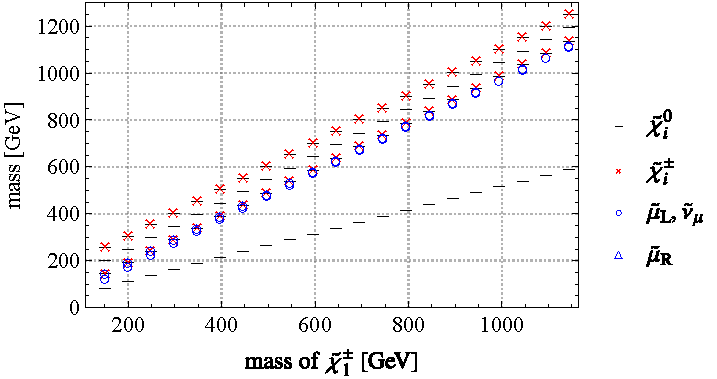
\includegraphics[height=85pt]{../plots/plot_tab1x095_mass.pdf}
  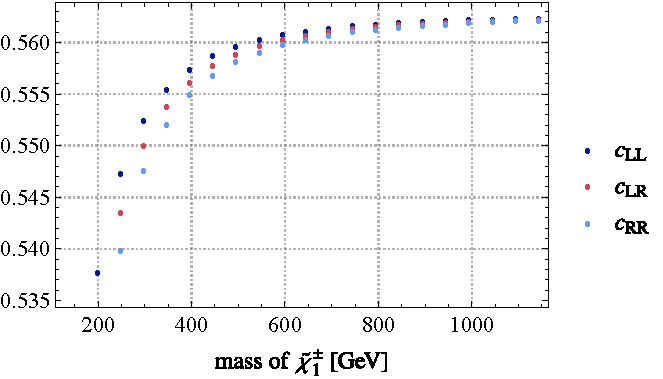
\includegraphics[height=85pt]{../plots/plot_tab1x095_cfactors.pdf}
\par
  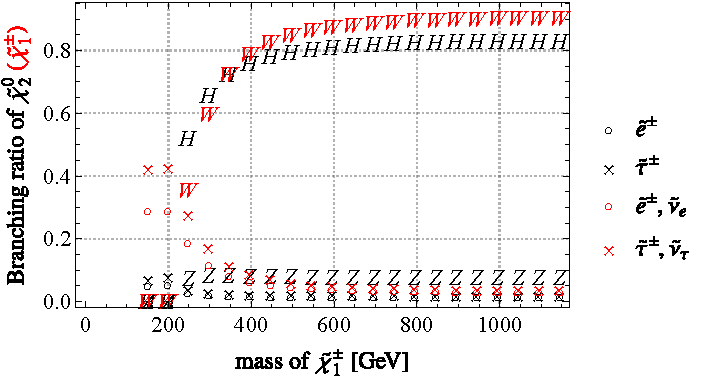
\includegraphics[height=85pt]{../plots/plot_tab1x095_br21.pdf}
  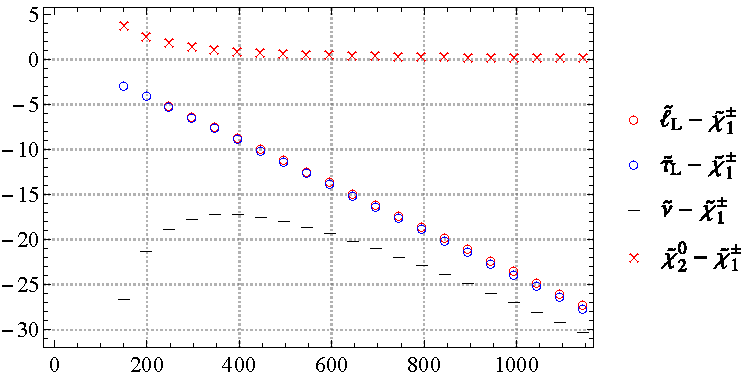
\includegraphics[height=85pt]{../plots/plot_tab1x095_massdiff.pdf}
\par
  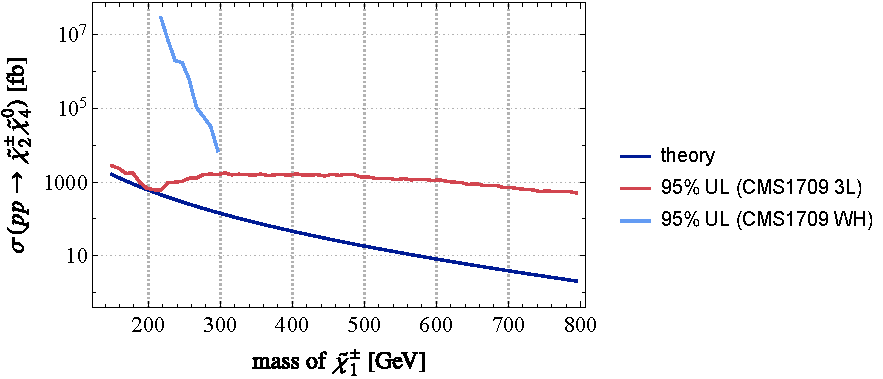
\includegraphics[height=90pt]{../plots/plot_tab1x095_limit21.pdf}
  \caption{\label{fig:tab1x095}The property of tab1-0.95 benchmark line. The models are generated with $M_2=200,250,\dots,1200\GeV$, while $m_{\charPM[1]}$ is used as labels.\\
 (A) Masses of relevant SUSY particles. Note that $\tilde\mu\w R$ is decoupled.
 (B) The cross-section $c$-factor (see \texttt{analysis.pdf}).
 (C) The BRs of $\charPM[1]$ (red) and $\neut[2]$ (black).\\
 (D) The mass differences between SUSY particles. The LSP is  $\tilde\nu$ for $m_{\charPM[1]}\lesssim 500\GeV$.\\
 (E) The theoretical cross section of $pp\to\charPM[1]\neut[2]$ and interpreted upper limits on it.
}
\end{figure}

On this line, $\neut[2]$ has very small BRs to $\tilde\ell$ or $Z$; because of the phase space suppression, it mainly decays to $H\neut[1]$ for $m_{\charPM[1]}\gtrsim250\GeV$ and to $\tilde\nu\nu$ for $m_[\charPM[1]]\lesssim250\GeV$.
Therefore, CMS1709 (b) and (c) does not give any limits as far as we consider $\neut[2]\charPM[1]$ production.
Meanwhile, the search for $WH+\mET$, i.e., (e) gives very weak constraints.
So we cannot constrain the models on this line in this study.

In actual experiments, the models should be covered by CMS1709 (b) and (c) because of the events from $pp\to\neut[4]\charPM[2]$.
Our study cannot cover this process because they have smaller $x$; it requires MC simulation.
However, assuming that $x$ closer to 0.5 should give better $\mathcal A\times\mathcal E$, we can give a conservative upper limit on $\sigma(pp\to\neut[4]\charPM[2])$ with using the CMS upper limits for $x=0.95$.
The result is shown in \cref{fig:tab1x005N4C2}; $K_\Gamma$ and $K_\sigma$ for $\neut[4]\charPM[2]$ are prepared, and $\sigma_{\text{CMS1709a;$x=0.95$}}$ is used (and hence the limit is very conservative).
Accordingly, the lower bound  of 150--200\,GeV on $m_{\charPM[1]}$ is observed.

\begin{figure}[b]
  \centering
  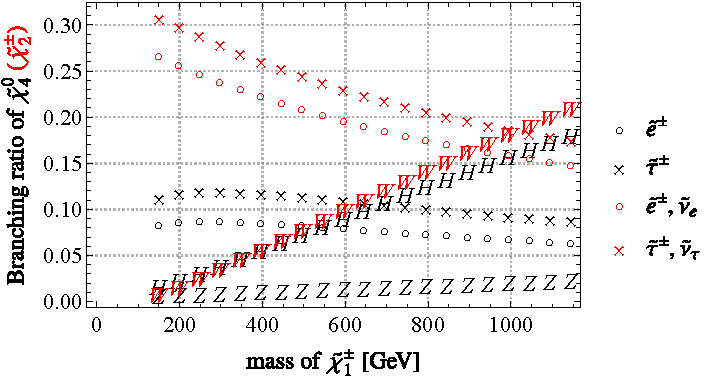
\includegraphics[height=80pt]{../plots/plot_tab1x095_br42.pdf}
  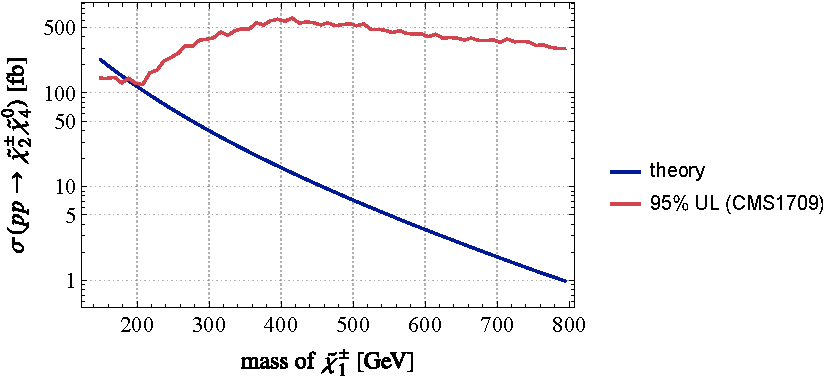
\includegraphics[height=80pt]{../plots/plot_tab1x095_limit42.pdf}

  \caption{\label{fig:tab1x095N4C2}The extra property of tab1-0.50 benchmark line.
 (A) The BRs of $\charPM[2]$ (red) and $\neut[4]$ (black).
 (B) The theoretical cross section of $pp\to\charPM[2]\neut[4]$ and interpreted upper limits on it.
}
\end{figure}

\clearpage

\subsection{tab1-bosonic}

This is the models where $\neut$ and $\charPM$ decays mainly to $W^\pm+\neut[1]$ and $(Z\text{ or }H)+\neut[1]$, respectively, which is typically realized when sleptons are heavier than wino/higgsino.
As a benchmark line, we use the models characterized by
\begin{equation}
 M_2=\mu=2M_1,
\quad
 m^2_L=(1200\GeV)^2,
\quad
 \tan\beta=40,
\quad
 \tilde l\w R, \tilde q, \text{heavy-Higgs: decoupled}
\end{equation}
with $M_2<1000\GeV$.

\begin{figure}[h]
  \centering
  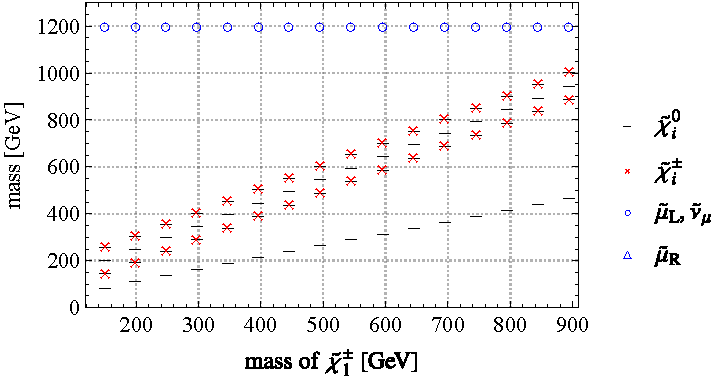
\includegraphics[height=90pt]{../plots/plot_tab1boson_mass.pdf}
  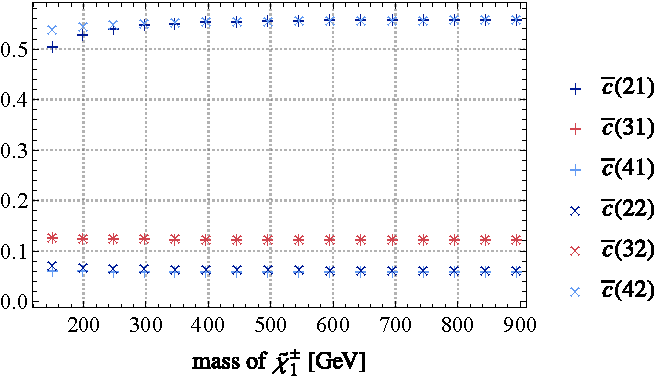
\includegraphics[height=90pt]{../plots/plot_tab1boson_cfactors.pdf}
\par
  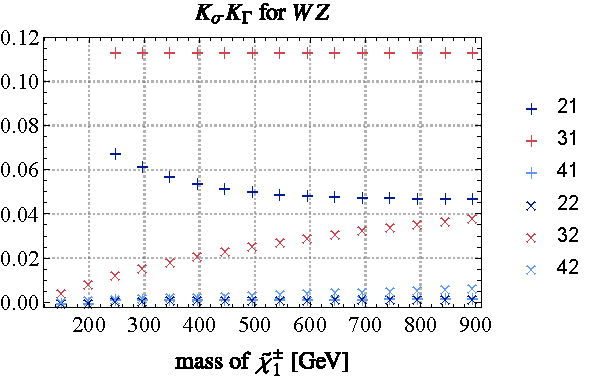
\includegraphics[height=90pt]{../plots/plot_tab1boson_WZ.pdf}
  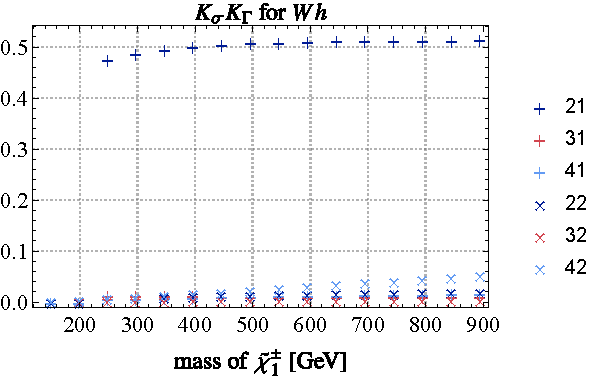
\includegraphics[height=90pt]{../plots/plot_tab1boson_WH.pdf}
\par
  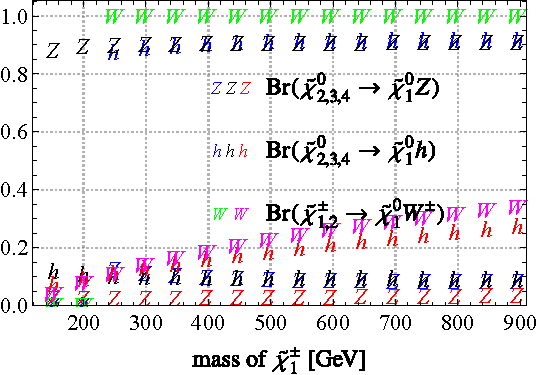
\includegraphics[height=90pt]{../plots/plot_tab1boson_br.pdf}
  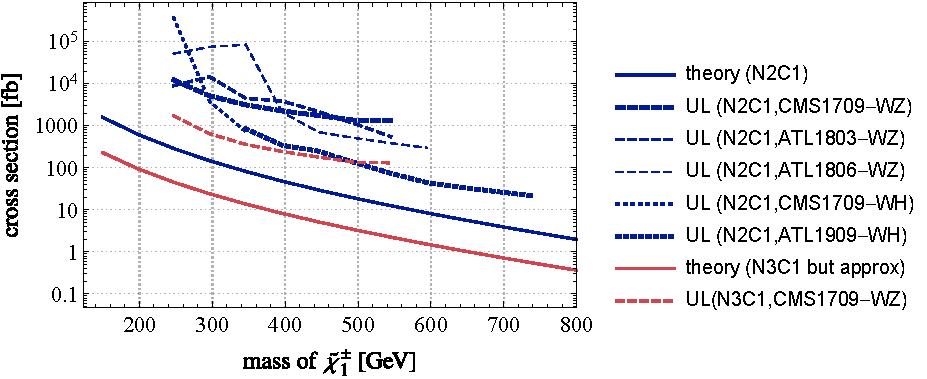
\includegraphics[height=90pt]{../plots/plot_tab1boson_limit.pdf}
  \caption{\label{fig:tab1x095}The property of tab1-boson benchmark line. The models are generated with $M_2=200,250,\dots,950\GeV$, while $m_{\charPM[1]}$ is used as labels.\\
 (A) Masses of relevant SUSY particles. Note that $\tilde\mu\w R$ is decoupled.\\
 (B) The cross-section $c$-factor for $\charPM[1]\neut[2]$ (see \texttt{analysis.pdf}).\\
 (C) The neutralino/chargino BRs.\\
 (D) The theoretical cross section of $pp\to\charPM[1]\neut[2]$ and interpreted upper limits on it based on CMS1709. In addition, $\sigma\w{UL}$ for $\charPM[1]\neut[3]$ process is obtained with extra simplification (see text).
}
\end{figure}


The mass spectrum is shown in \cref{fig:tab1x050}; we use $m_{\charPM[1]}$ to label each model point.
For $m_{\charPM[1]}<200\GeV$, the bosonic process is kinematically forbidden (as we studied before) and thus we do not consider the region.

The main target, $\neut[2]\charPM[1]$ process, has a sizable $K_\sigma\sim0.56$, but it mainly results in $WH+\mET$.
As we observe in the last figure, $WZ+\mET$ search does not give any limit (because of smaller $K_\Gamma$) and $WH+\mET$ search does neither (because of weak $\sigma\w{UL;CMS}$).

In fact, $WZ+\mET$ signature is mainly generated by $pp\to\neut[3]\charPM[1]$ process.
We consider this process, neglecting the mass difference of $\neut[3]$--$\charPM[1]$, the production cross section difference, and the acceptance/efficiency difference.
No constraints are obtained, though, as shown in the red lines of the last plot, which is because it is (a kind of) higgsino-production and its $K_\sigma\sim0.12$ is 4--5 times smaller than $\neut[2]\charPM[1]$.

In summary, tab1-bosonic models are not constrained by ATL1803/CMS1709 analysis.\footnote{The compressed models ($m_{\charPM[1]}\lesssim200\GeV$) are expected to be fully excluded, considering our previous study, but we do not provide quantitative discussion in this work.}

\subsection{tab1-slep}

In addition to the above four lines, the parameter space is directly constrained by searches for slepton pair-production (i.e., ATLAS 1908).
We should compare
\begin{equation}
 \sigma_X\cdot\Br(\tilde\mu\to\mu\neut[1])^2\text{~v.s.~}\sigma_{\text{UL;original;left-only}}
\end{equation}
for each benchmark point, giving the red squares (black dots) as the excluded (not excluded\footnote{Note that these not-excluded points may have been excluded by the original analysis (ATLAS1908) thanks to contributions from cascade decays.}) in \cref{fig:tab1-summary}.

\subsection{tab1-summary}
Combining all the analyses, we may draw some figures like \cref{fig:tab1-summary}.

\begin{figure}[h]\centering
  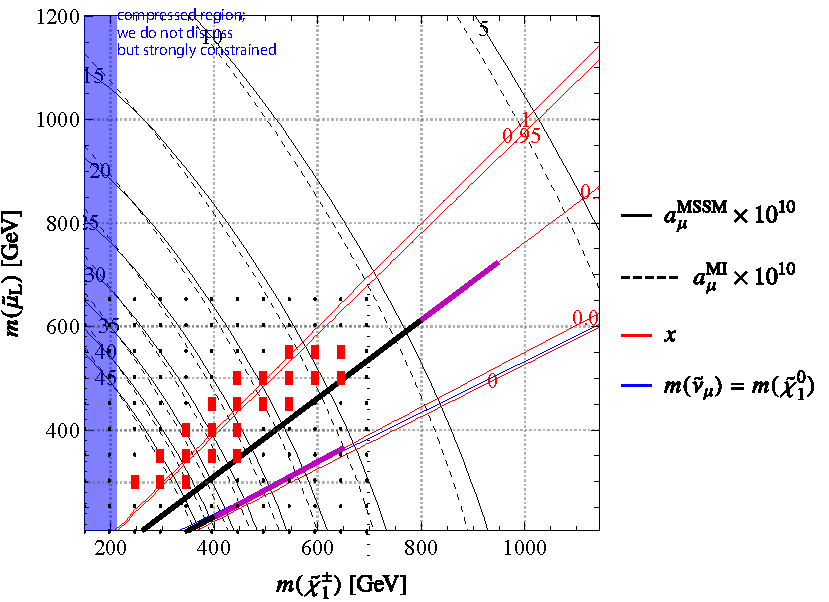
\includegraphics[height=300pt]{mueqm2.pdf}
  \caption{\label{fig:tab1-summary}The summary plot for ``tab1'', i.e.,
 $\mu=M_2=2M_1$, $\tan\beta=40$, decoupled-$m_{\tilde l\w R}$, flavor universal.
 The signatures NC/WZ, NC/WH, CC/WW, SLSL are analyzed in the whole parameter space but only SLSL signature gives constraints (red squares as excluded, black dots as survived).
 NC/3L and NC/LLT are analyzed only on the $x=0.05, 0.5, 0.95$ lines; black/purple thick line as ``certainly''/''possibly'' excluded, where no constraints are obtained for $x=0.95$.
 Compressed region ($\max(m_{\neut[2]}-m_Z,m_{\charPM[1]}-m_W)<m_{\neut[1]}$) are not studied but  it should be mostly excluded.
 In all the analyses, contributions from cascade decays are not considered at all.
}
\end{figure}


\clearpage
\subsection[tab2:mu=2M2]{tab2: $\mu=2M_2$}
The analysis is repeated for $\mu=M_2$, as shown in the summary plot \cref{fig:tab22-summary}.
Figures of each analysis are also given below.

\begin{figure}[h]\centering
  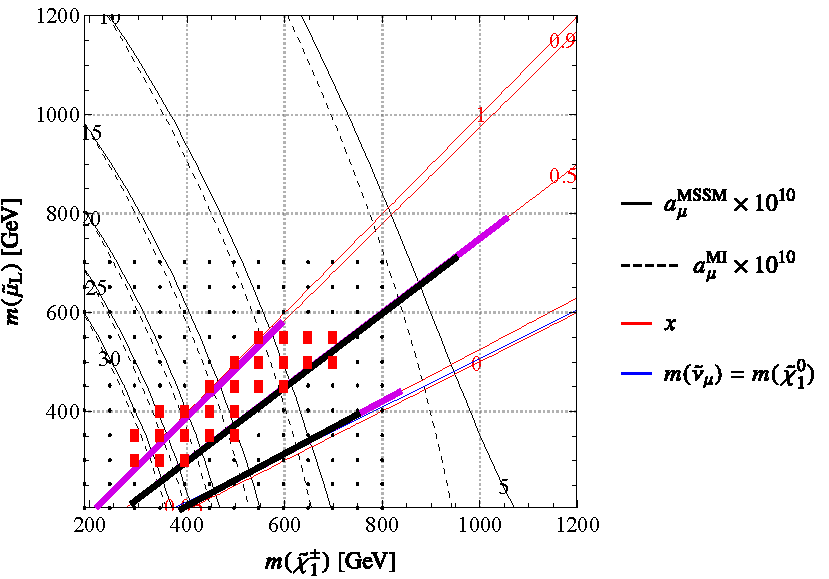
\includegraphics[height=250pt]{mueq2m2.pdf}
  \caption{\label{fig:tab2-summary}The summary plot for ``tab2'', i.e.,
 $\mu=2M_2=4M_1$, $\tan\beta=40$, decoupled-$m_{\tilde l\w R}$, flavor universal.
 The signatures NC/WZ, NC/WH, CC/WW, SLSL are analyzed in the whole parameter space but only SLSL signature gives constraints (red squares as excluded, black dots as survived).
 NC/3L and NC/LLT are analyzed only on the $x=0.05, 0.5, 0.95$ lines; black/purple thick line as ``certainly''/''possibly'' excluded, where no constraints are obtained for $x=0.95$.
 Compressed region ($\max(m_{\neut[2]}-m_Z,m_{\charPM[1]}-m_W)<m_{\neut[1]}$) are not in this plot range.
 In all the analyses, contributions from cascade decays are not considered at all.
}
\end{figure}


\subsubsection{$x=0.50$}

\begin{figure}[h!]\centering
  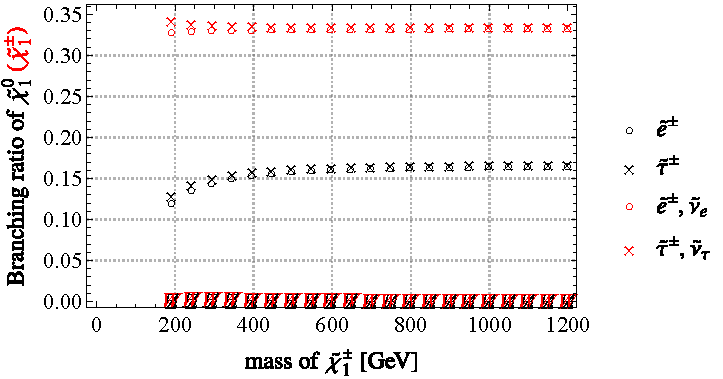
\includegraphics[height=80pt]{../plots/plot_tab2x050_br21.pdf}
  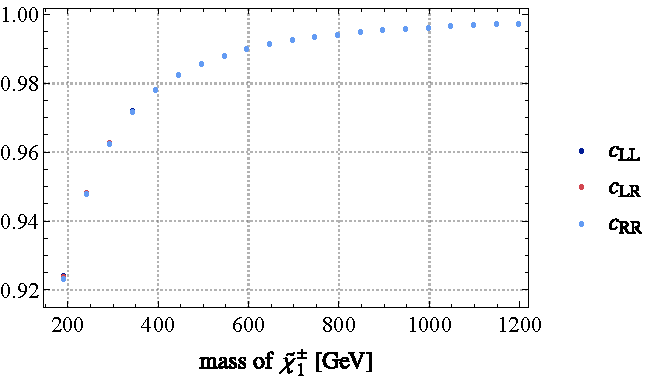
\includegraphics[height=80pt]{../plots/plot_tab2x050_cfactors.pdf}\par
  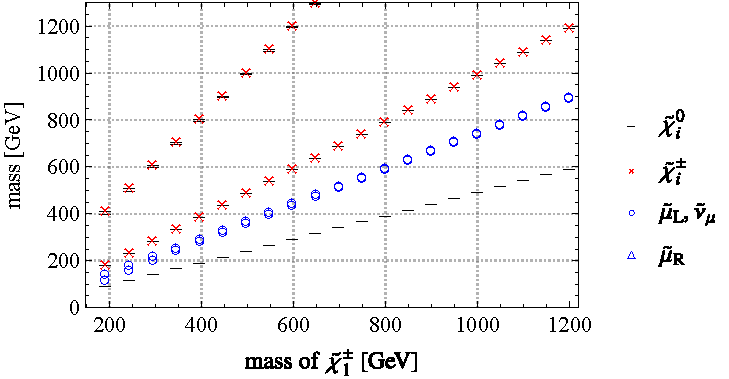
\includegraphics[height=80pt]{../plots/plot_tab2x050_mass.pdf}
  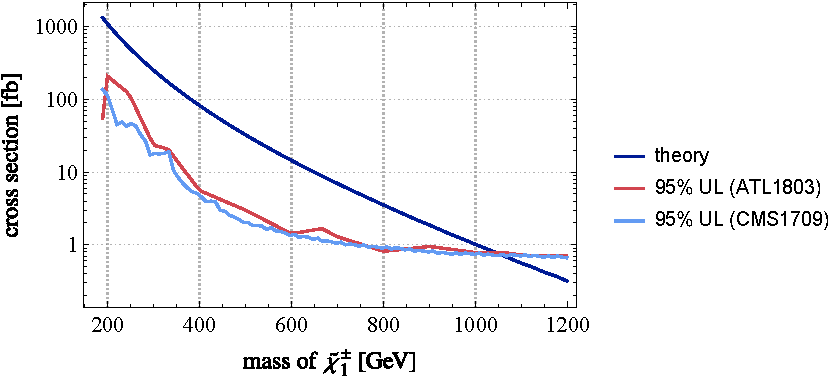
\includegraphics[height=80pt]{../plots/plot_tab2x050_limit.pdf}
\end{figure}

\clearpage

\subsubsection{$x=0.05$}

\begin{figure}[h!]\centering
  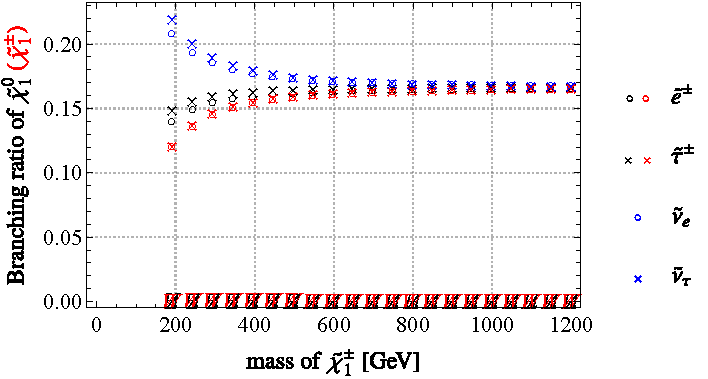
\includegraphics[height=80pt]{../plots/plot_tab2x005_br21.pdf}
  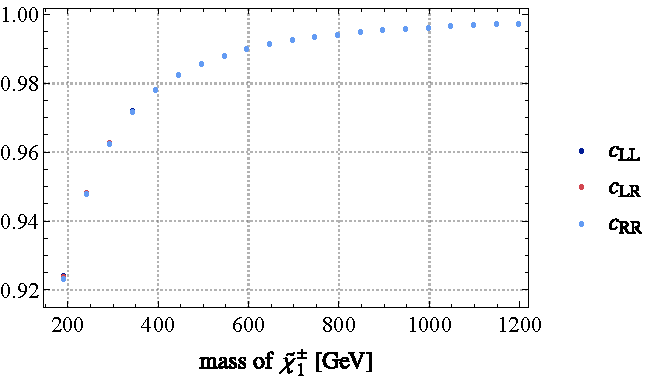
\includegraphics[height=80pt]{../plots/plot_tab2x005_cfactors.pdf}\par
  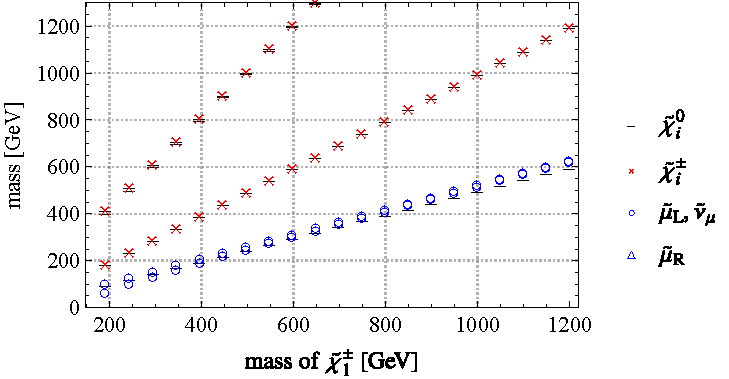
\includegraphics[height=80pt]{../plots/plot_tab2x005_mass.pdf}
  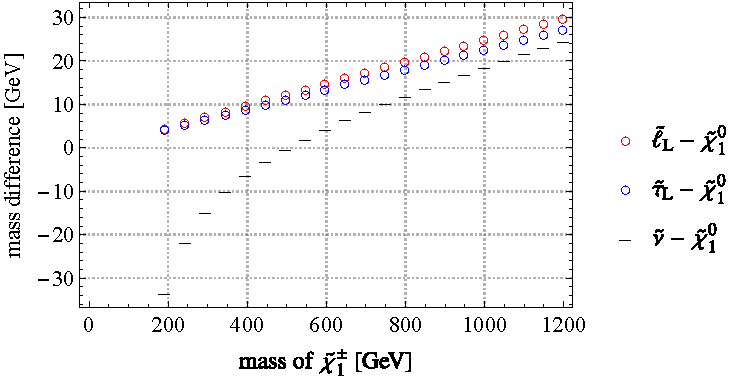
\includegraphics[height=80pt]{../plots/plot_tab2x005_massdiff.pdf}\par
  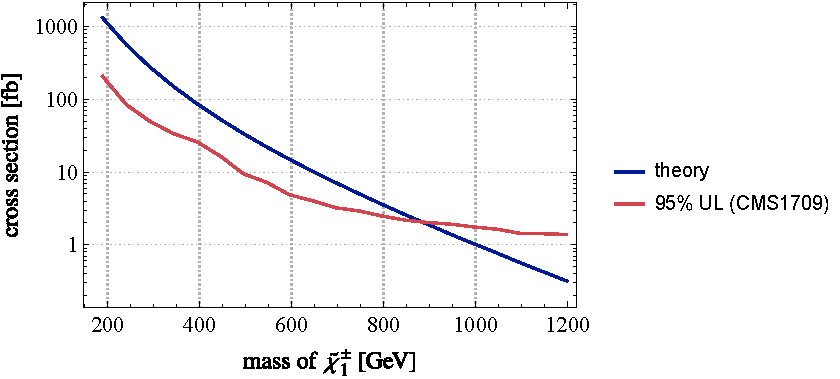
\includegraphics[height=80pt]{../plots/plot_tab2x005_limit.pdf}
\end{figure}

\subsubsection{$x=0.95$}

\begin{figure}[h!]\centering
  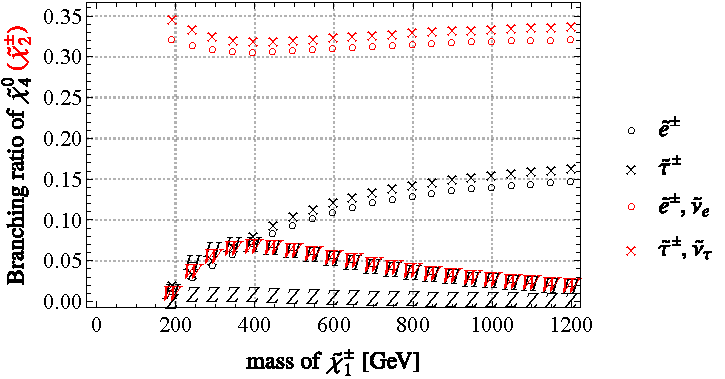
\includegraphics[height=80pt]{../plots/plot_tab2x095_br21.pdf}
  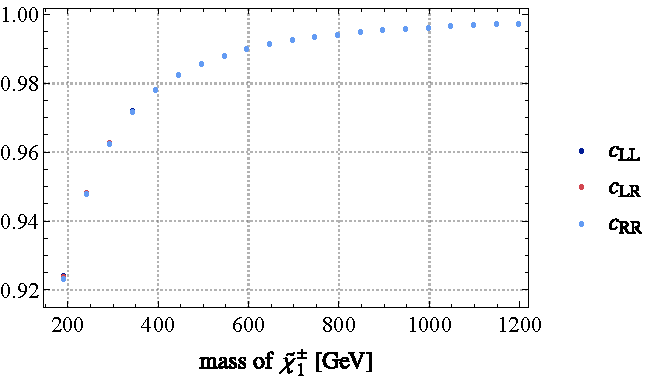
\includegraphics[height=80pt]{../plots/plot_tab2x095_cfactors.pdf}\par
  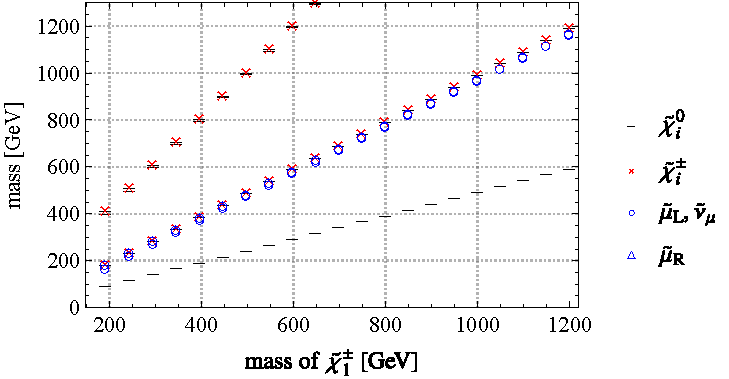
\includegraphics[height=80pt]{../plots/plot_tab2x095_mass.pdf}
  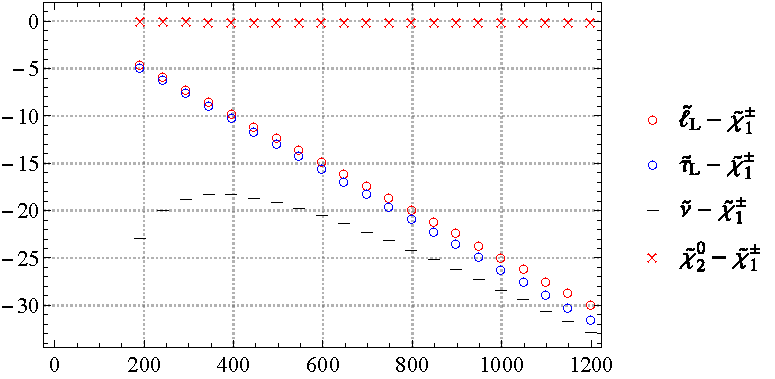
\includegraphics[height=80pt]{../plots/plot_tab2x095_massdiff.pdf}\par
  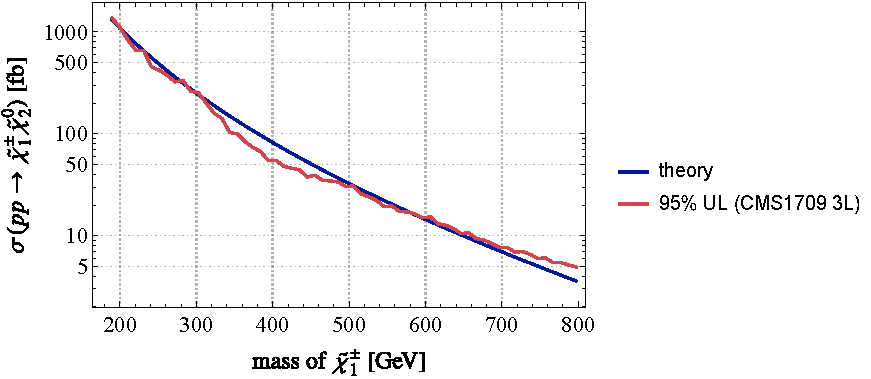
\includegraphics[height=80pt]{../plots/plot_tab2x095_limit21.pdf}
\end{figure}

\clearpage
\subsubsection{bosonic decay cases (heavier sleptons)}

\begin{figure}[h!]\centering
  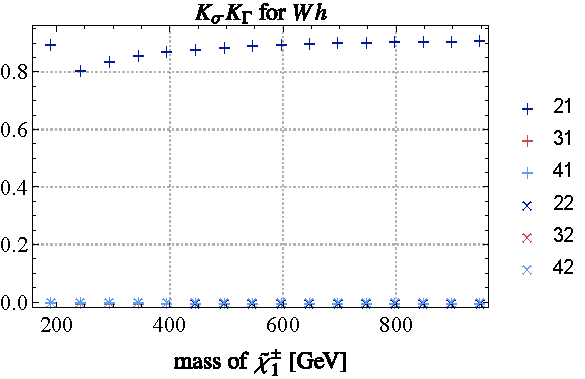
\includegraphics[height=110pt]{../plots/plot_tab2boson_WH.pdf}
  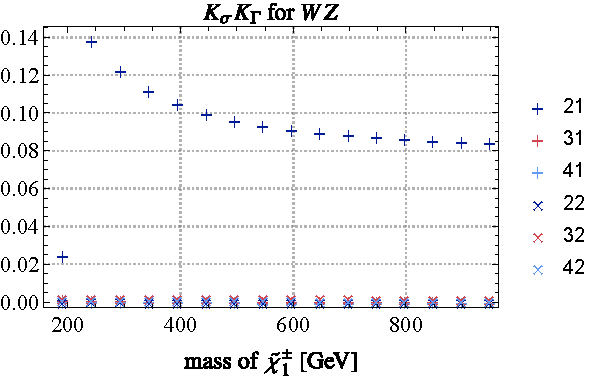
\includegraphics[height=110pt]{../plots/plot_tab2boson_WZ.pdf}
  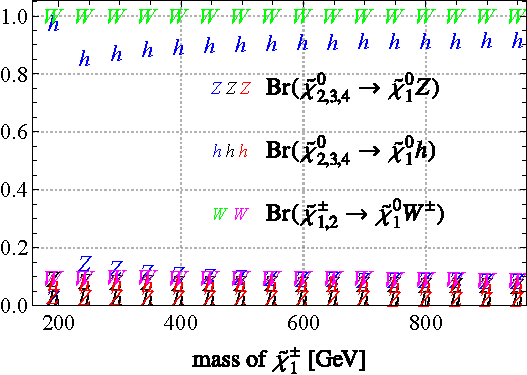
\includegraphics[height=110pt]{../plots/plot_tab2boson_br.pdf}
  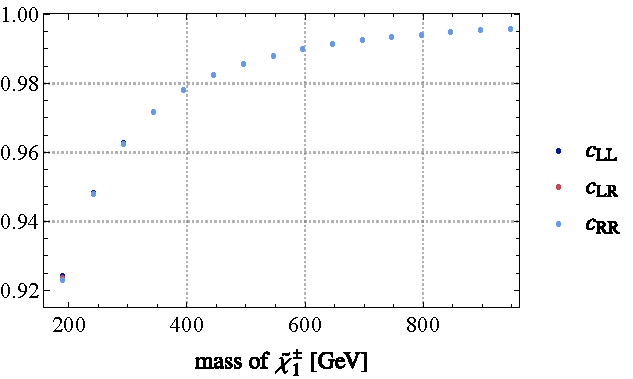
\includegraphics[height=110pt]{../plots/plot_tab2boson_cfactors.pdf}
  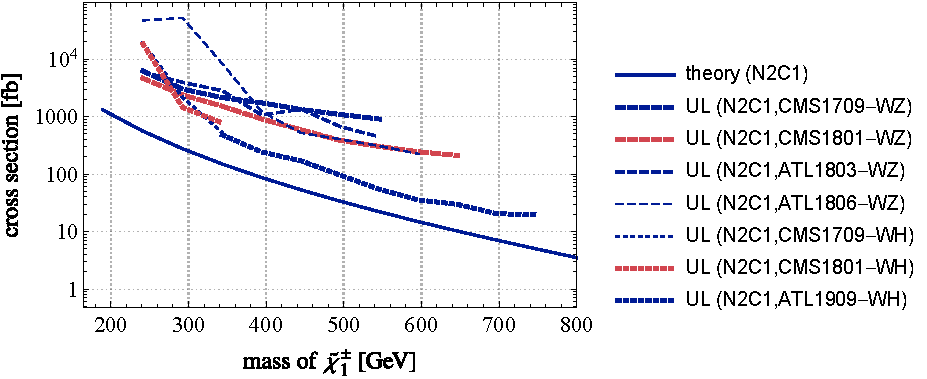
\includegraphics[height=110pt]{../plots/plot_tab2boson_limit.pdf}
  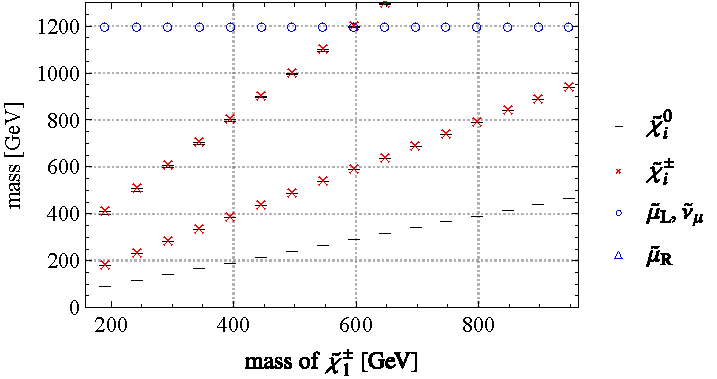
\includegraphics[height=110pt]{../plots/plot_tab2boson_mass.pdf}
\end{figure}

\subsubsection{slepton bound}
\begin{figure}[h!]\centering
  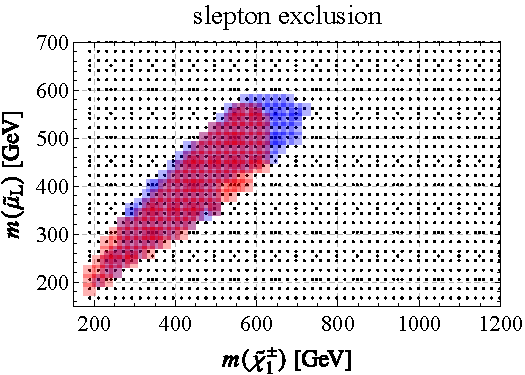
\includegraphics[height=120pt]{../plots/plot_tab2slep_limit.pdf}
\end{figure}

\clearpage
\subsection{100GeV LSP tab1 grid}
The situation is simpler than the previous cases.

\begin{figure}[h!]\centering
  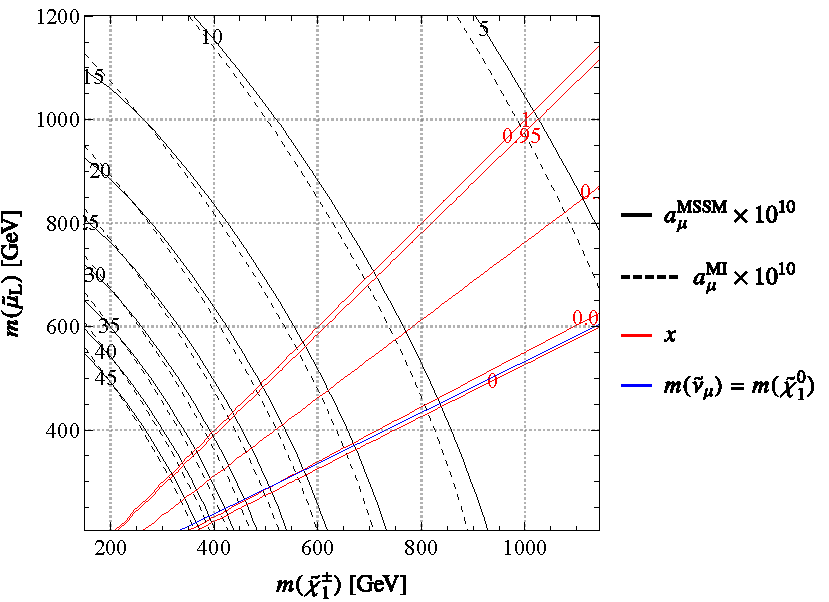
\includegraphics[height=150pt]{../plots/plot_spectrum_tab1_physplot.pdf}
  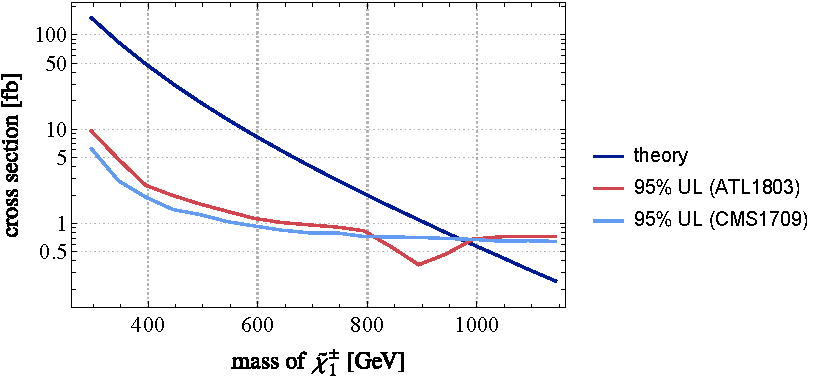
\includegraphics[height=90pt]{../plots/plot_tab1m100x050_limit.pdf}
  \includegraphics[height=90pt]{../plots/plot_tab1m100x005_limit.pdf}
  \includegraphics[height=90pt]{../plots/plot_tab1m100x095_limit21.pdf}
  \includegraphics[height=110pt]{../plots/plot_tab1m100boson_limit.pdf}
  \includegraphics[height=110pt]{../plots/plot_tab1m100slep_limit.pdf}
\caption{Results for $m_{\neut[1]}=100\GeV$, $\mu=M_2$. Each plot shows physical parameters,  limits at $x=0.05$, 0.50, and 0.95, bosonic limits (i.e., $m_{\tilde l_L}>m_{\charPM[1],\neut[2]}$), and constraints from slepton pair-production.}
\end{figure}

\clearpage
\subsubsection{Supporting figures}
\begin{figure}[h!]\centering
 \includegraphics[height=60pt]{../plots/plot_tab1m100x005_mass.pdf}
 \includegraphics[height=60pt]{../plots/plot_tab1m100x005_massdiff.pdf}
 \includegraphics[height=60pt]{../plots/plot_tab1m100x005_cfactors.pdf}
 \includegraphics[height=60pt]{../plots/plot_tab1m100x005_br21.pdf}
\caption{Supporting figures for tab1m100 $x=0.05$ line.}
\end{figure}
\begin{figure}[h!]\centering
 \includegraphics[height=60pt]{../plots/plot_tab1m100x050_mass.pdf}
 \includegraphics[height=60pt]{../plots/plot_tab1m100x050_cfactors.pdf}
 \includegraphics[height=60pt]{../plots/plot_tab1m100x050_br21.pdf}
\caption{Supporting figures for tab1m100 $x=0.50$ line.}
\end{figure}
\begin{figure}[h!]\centering
 \includegraphics[height=60pt]{../plots/plot_tab1m100x095_br21.pdf}
 \includegraphics[height=60pt]{../plots/plot_tab1m100x095_cfactors.pdf}
 \includegraphics[height=60pt]{../plots/plot_tab1m100x095_mass.pdf}
 \includegraphics[height=60pt]{../plots/plot_tab1m100x095_massdiff.pdf}
\caption{Supporting figures for tab1m100 $x=0.95$ line.}
\end{figure}
\begin{figure}[h!]\centering
 \includegraphics[height=60pt]{../plots/plot_tab1m100boson_cfactors.pdf}
 \includegraphics[height=60pt]{../plots/plot_tab1m100boson_br.pdf}
 \includegraphics[height=60pt]{../plots/plot_tab1m100boson_WZ.pdf}
 \includegraphics[height=60pt]{../plots/plot_tab1m100boson_WH.pdf}
\caption{Supporting figures for tab1m100 boson limit.}
\end{figure}

\clearpage
\subsection{100GeV LSP tab2 grid}

\begin{figure}[h!]\centering
  \includegraphics[height=150pt]{../plots/plot_spectrum_tab2_physplot.pdf}
  \includegraphics[height=90pt]{../plots/plot_tab2m100x050_limit.pdf}
  \includegraphics[height=90pt]{../plots/plot_tab2m100x005_limit.pdf}
  \includegraphics[height=90pt]{../plots/plot_tab2m100x095_limit21.pdf}
  \includegraphics[height=110pt]{../plots/plot_tab2m100boson_limit.pdf}
  \includegraphics[height=110pt]{../plots/plot_tab2m100slep_limit.pdf}
\caption{Results for $m_{\neut[1]}=100\GeV$, $\mu=2M_2$. Each plot shows physical parameters,  limits at $x=0.05$, 0.50, and 0.95, bosonic limits (i.e., $m_{\tilde l_L}>m_{\charPM[1],\neut[2]}$), and constraints from slepton pair-production.}
\end{figure}

\clearpage
\subsubsection{Supporting figures}
\begin{figure}[h!]\centering
 \includegraphics[height=60pt]{../plots/plot_tab2m100x005_mass.pdf}
 \includegraphics[height=60pt]{../plots/plot_tab2m100x005_massdiff.pdf}
 \includegraphics[height=60pt]{../plots/plot_tab2m100x005_cfactors.pdf}
 \includegraphics[height=60pt]{../plots/plot_tab2m100x005_br21.pdf}
\caption{Supporting figures for tab2m100 $x=0.05$ line.}
\end{figure}
\begin{figure}[h!]\centering
 \includegraphics[height=60pt]{../plots/plot_tab2m100x050_mass.pdf}
 \includegraphics[height=60pt]{../plots/plot_tab2m100x050_cfactors.pdf}
 \includegraphics[height=60pt]{../plots/plot_tab2m100x050_br21.pdf}
\caption{Supporting figures for tab2m100 $x=0.50$ line.}
\end{figure}
\begin{figure}[h!]\centering
 \includegraphics[height=60pt]{../plots/plot_tab2m100x095_br21.pdf}
 \includegraphics[height=60pt]{../plots/plot_tab2m100x095_cfactors.pdf}
 \includegraphics[height=60pt]{../plots/plot_tab2m100x095_mass.pdf}
 \includegraphics[height=60pt]{../plots/plot_tab2m100x095_massdiff.pdf}
\caption{Supporting figures for tab2m100 $x=0.95$ line.}
\end{figure}
\begin{figure}[h!]\centering
 \includegraphics[height=60pt]{../plots/plot_tab2m100boson_cfactors.pdf}
 \includegraphics[height=60pt]{../plots/plot_tab2m100boson_br.pdf}
 \includegraphics[height=60pt]{../plots/plot_tab2m100boson_WZ.pdf}
 \includegraphics[height=60pt]{../plots/plot_tab2m100boson_WH.pdf}
\caption{Supporting figures for tab2m100 boson limit.}
\end{figure}

\clearpage
\bibliography{analysis}
\end{document}
